\subsection{Descrizione del task}
La \textbf{classificazione del testo}, conosciuta anche come \textit{tagging del testo} o \textit{categorizzazione del testo}, è il processo di categorizzazione dei corpora in gruppi organizzati. Utilizzando il Natural Language Processing, i classificatori possono analizzare automaticamente i testi e poi assegnare loro un insieme di tag o categorie predefinite in base al suo contenuto. \citet{textclassificationproblem_stanford}, ricercatori della Stanford University, definiscono il problema nella maniera seguente. 

Nella classificazione del testo, ci viene data una descrizione \(d\in \mathbb{X}\) di un documento, dove \(\mathbb{X}\) è lo \textit{spazio dei documenti}, e un insieme fissato di \textit{classi} \(\mathbb{C}={c_1,c_2,...,c_j}\), chiamate anche \textit{categorie} o \textit{etichette}. Tipicamente, lo spazio dei documenti \(\mathbb{X}\) è un qualche tipo di spazio di grandi dimensioni (high-dimensional space), e le classi sono definite dall'uomo per la necessità di una specifica applicazione. Ci viene fornito anche un insieme per l'addestramento \(\mathbb{D}\) di documenti etichettati \(\langle d,c \rangle \in \mathbb{X} \times \mathbb{C}\).
Per esempio:
\begin{center}
\(\langle d,c \rangle\) = \(\langle\) Pechino entra nell'Organizzazione Mondiale del Commercio, China \(\rangle\)
\end{center}
per il documento \textit{Pechino entra nell'Organizzazione Mondiale del Commercio} e la classe \textit{China}.

Utilizzando un \textit{algoritmo di apprendimento}, vogliamo poi creare un classificatore o una \textit{funzione di classificazione} \(\gamma\) che mappa documenti in classi:
\begin{center}
\(\gamma:\mathbb{X}\rightarrow\mathbb{C}\)
\end{center}

Questo tipo di apprendimento è chiamato \textbf{apprendimento supervisionato} perché un supervisore (la persona che definisce le classi ed etichetta i documenti utilizzati per l'addestramento) serve come un \textit{insegnante} che dirige il processo di apprendimento. Per il momento, consideriamo solo i problemi \textit{one-of} in cui un documento è membro esattamente di una classe: il nostro obiettivo nella classificazione del testo è un'alta accuratezza sui dati di test. 

La classificazione del testo sta diventando una parte sempre più importante nelle aziende, poiché permette di ottenere facilmente informazioni dai dati e automatizzare i processi aziendali. Alcuni degli esempi e dei casi d'uso più comuni per la classificazione automatica del testo sono i seguenti:

\begin{itemize}
    \item \textbf{Sentiment Analysis}: il processo di capire se un dato testo sta parlando positivamente o negativamente di un dato argomento (ad esempio per scopi di monitoraggio del marchio).
    \item \textbf{Language Detection}: la procedura di rilevamento della lingua di un dato testo (ad esempio sapere se un ticket di supporto in arrivo è scritto in inglese o in spagnolo per indirizzarlo automaticamente al team appropriato).
    \item \textbf{Topic Detection}: il compito di identificare il tema o l'argomento di una porzione di testo (ad esempio, sapere se una recensione di un prodotto da parte di un cliente riguarda la facilità d'uso, il supporto clienti o il prezzo). Questo è il compito che è stato studiato durante la fase di analisi descritta in questo capitolo.
\end{itemize}

\begin{figure}[hbt!]
    \centering
    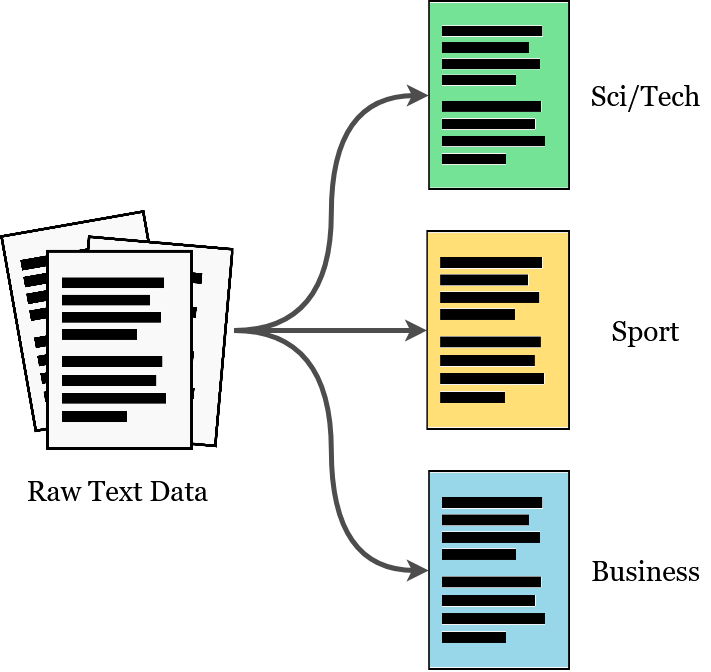
\includegraphics[width=0.5\textwidth]{img/textc_example.png}
    \caption{Text Classification: topic detection}
    \label{fig:textc_example}
\end{figure}